\documentclass[../main.tex]{subfiles}
\graphicspath{{\subfix{..}}}
\begin{document}
\chapter{Graph representation of JUNO for IBD reconstruction}
\epigraph{``The Answer to the Great Question of Life, the Universe and Everything is Forty-two''}{Douglas Adams, The Hitchhiker’s Guide to the Galaxy}
\label{sec:jgnn}
%\begin{itemize}
%  \item Introduce the concpet of reconstruction using Small + Large
%  \item Re state the context
%\end{itemize}

We previously showed, in chapter \ref{sec:jcnn}, that neural networks are relevant as reconstruction tools in JUNO. Even if they show worse performance, the combination to classical estimator could still bring improvement. We discussed the use of Convolutional Neural Network (CNN) in the previous chapter and their limitation, in particular the limitation of the image representation for the experiment.

In this chapter we propose to use a Graph Neural Network (GNN) to overcome those limitation.

\section{Motivation}
\label{sec:jgnn:motiv}
%\begin{itemize}
%  \item Problem with the image representation
%  \item Explain that graph can be a solution
%\end{itemize}

As explained in chapter \ref{sec:juno} the JUNO sensors, the Large Photomultipliers (LPMT) and Small Photomultipliers (SPMT), are arranged on a spherical plane, pointing to the center of the detector. When trying to represent this plane as a 2D image, due to the inherent problem of the projection, some part of the image are distorted and part of the image do not have any physical meaning (see section  \ref{sec:jcnn:data}). A way to represent the data without inducing deformation is the Graph, an object composed of a collection of nodes and a collection edges representing the relation between the nodes.

From this graph representation, we can construct a neural network that will process the data while keeping the properties of it. For example the rotational invariance, i.e. the energy and radius of the event do change if we rotate our referential. An approach was already proposed in JUNO by Qian et al. \cite{qian_vertex_2021} where each node of the graph are like pixels, they represent geometric region of the detector and are connected with their neighbours. The LPMT informations are then aggregated on those nodes. The network then process the data using the equivalent of convolution but on graph \cite{defferrard_convolutional_2017}.

In this work we want to take a step further in the graph representation by including the SPMT and including a maximum of raw informations.

\section{Data representation}
%\begin{itemize}
%  \item First though
%    \begin{itemize}
%      \item All pmt are nodes
%      \item How to connect ? Fully connected ?
%      \item Fully connected not possible with our computng capacities: 40k * 40k -> $1.6\cdot10^8$ link -> around a Gb of adjacency matrix times edges features
%      \item Connected to neighbours -> Already done for graph convolution, cit yury paper
%    \end{itemize}
%  \item Second though
%    \begin{itemize}
%      \item Be smarter
%      \item All PMTs as nodes -> Fired
%      \item Have intermediate layer of node representing geometric section -> Mesh
%      \item Fired connected to mesh
%      \item Mesh fully connected
%      \item Aggregation while keeping raw informations
%      \item Add a "global node"
%    \end{itemize}
%  \item Present healpix for the segementation
%  \item Features for node/edges
%    \begin{itemize}
%      \item Classic infos: Q,t,X,Y,Z (add plots to show features)
%      \item Add high order informations
%      \item Harmonic analysis (present here ? Or in annex ?)
%      \item Other high order $\mathcal{A}$ and $\mathcal{B}$
%    \end{itemize}
%  \item Difficulty: nodes do not live in the same space (not same infos on fired, mesh, and io)
%  \item Need a custom message passing options
%\end{itemize}

In an ideal world we would want to have every PMTs represented as node in the graph, each PMT being hit is an informations but the fact that PMTs were not hit is also an important information. It's by being aware of the whole of the system that we are able to give meaning to a subpart. As a reminder, in the Central Detector (CD), JUNO will posses 17612 LPMTs and 25600 SPMTs for a total of 43212 PMTs. This amount of information in itself is still manageable by modern computer if it were to be used in a neural network but when defining the relations between the nodes, it become a bit more tricky.

Excluding self relation, an edge that would go from and to the same node, and considering the relation to be undirected, the edge from $A$ to $B$ is the same from $B$ to $A$, the amount of edge is given by $\frac{n(n-1)}{2}$ which for 43212 PMTs amount for $933'616'866$ edges. If we encode an information with double precision (64 bits) in what we call an adjacency matrix, each information we want to encode in the relation would consume 4 GB of data. When adding the overhead due to gradient computation during training, this would put us over the memory capacity of a single V100 gpu card (20 GB of memory). We could use parallel training to distribute the training over multiple GPU but we considered that the technical difficulty to deploy this solution was not worth the trouble.

The option of connecting PMTs node only to their neighbours could be tempting to reduce the number of edge, but this solution does not translate well in term of internal representation in memory. Edges of sparsely connected nodes can be stored in efficient manner in a sparse matrix but the calculation in itself would often results in the concretization of the full matrix in memory, resulting in an insufficient memory gain during training.


We finally decided of a middle ground where:
\begin{itemize}
  \item The core of the graph will be composed of nodes representing geometric regions of the detector. We call those nodes {\color{Dandelion} mesh} node. Those mesh nodes are densely connected to each other. We keep their number of the order of magnitude of a thousand to keep the memory consumption low
  \item All the fired PMTs, PMTs that have been hit, will be represented as nodes. We call those node {\color{red} fired}. Fired nodes are connected to the mesh they geometrically belong.
  \item A final node which will hold global information about the detector and on which we will read the interaction vertex and energy. It's designated as the {\color{blue} I/O} node for input/output. This node will be connected to every mesh nodes.
\end{itemize}
Those nodes and their relations are illustrated in figure \ref{fig:jgnn:node_schema}. From this representation, we end up with three distinct adjacency adjacency matrix
\begin{itemize}
  \item A $N_{fired} \times N_{mesh}$ adjacency matrix, representing the relations between fired and mesh. Those relations are undirected.
  \item A $N_{mesh} \times N_{mesh}$ adjacency matrix, representing the relation between meshes. Those relation are directed.
  \item A $N_{mesh} \times 1$ adjacency between the mesh and I/O nodes. Those relations are undirected.
\end{itemize}
The adjacency matrix representing those relation is illustrated in figure \ref{fig:jgnn:adj}.

\begin{figure}
  \centering
  \begin{subfigure}[t]{0.48\linewidth}
    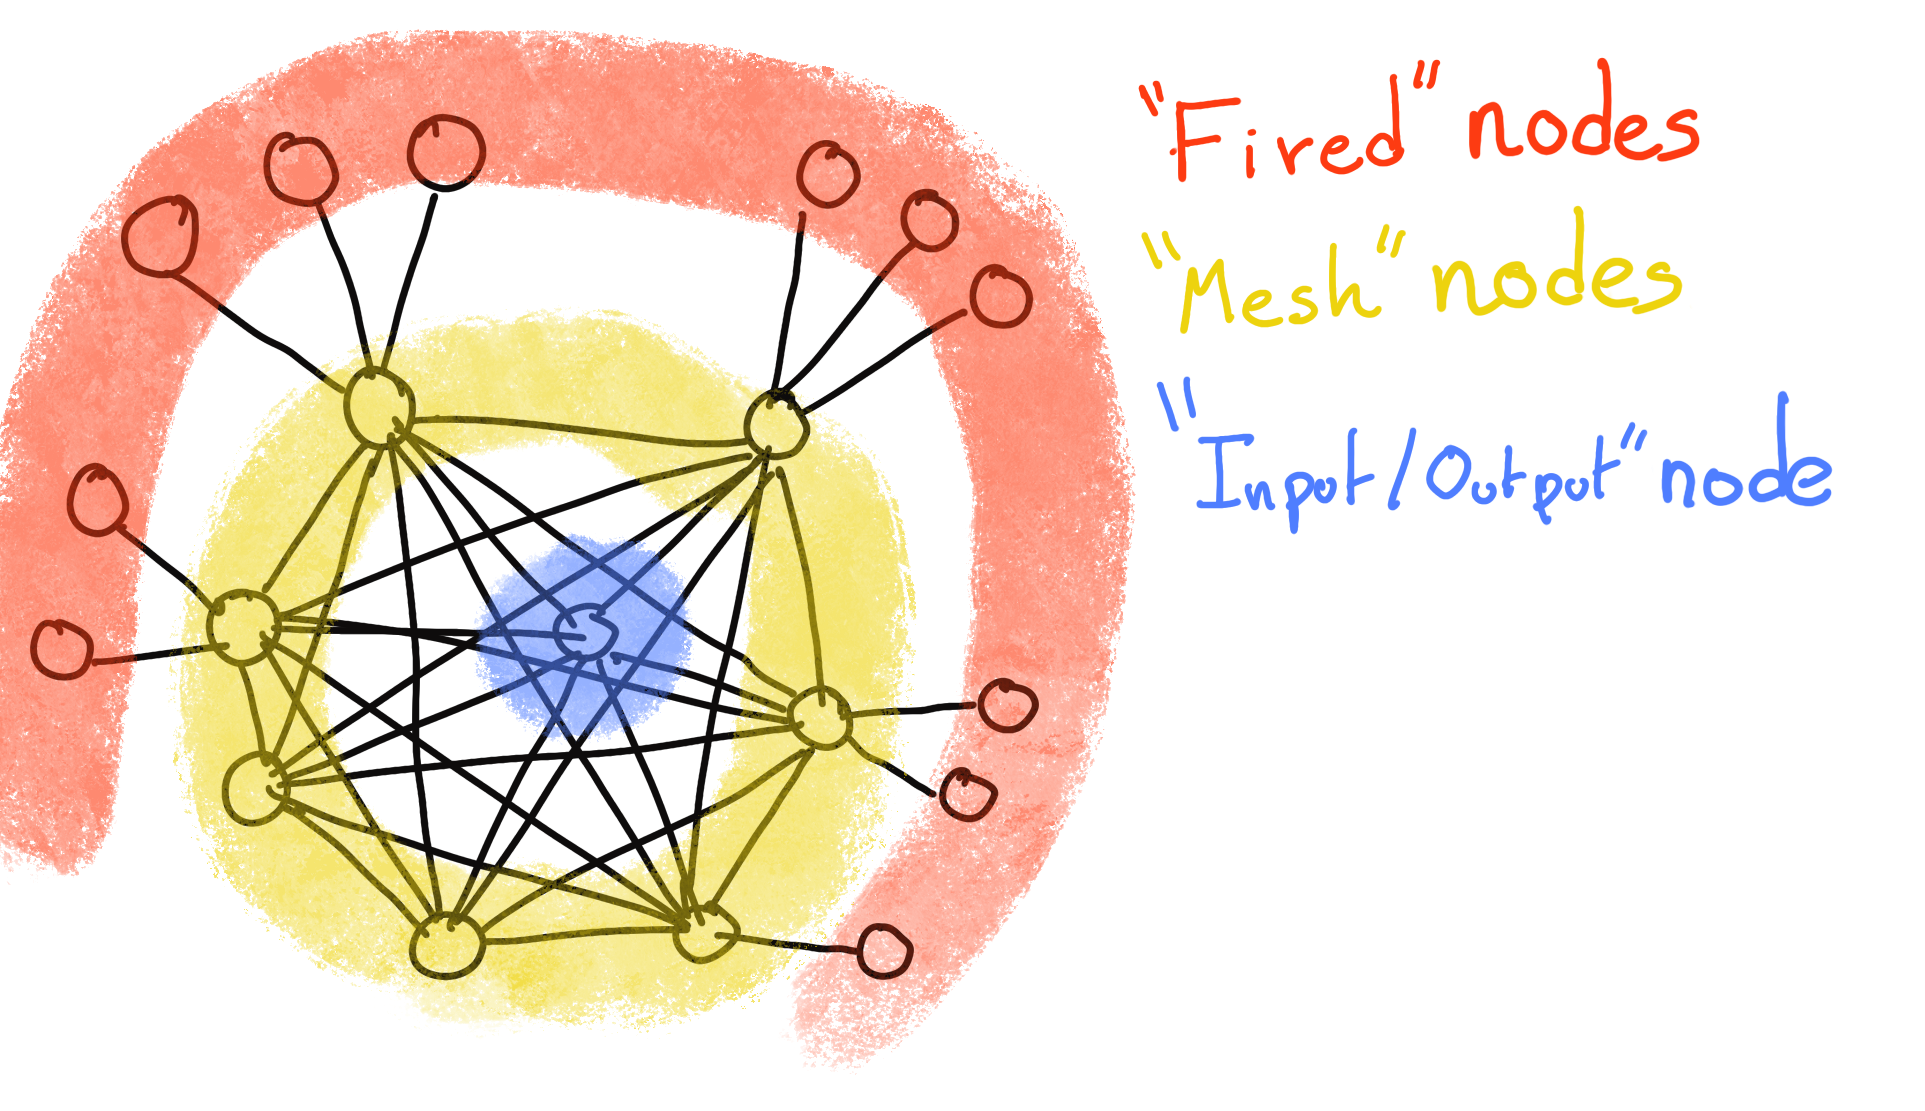
\includegraphics[width=\linewidth]{images/jgnn/nodes_schema.png}
    \caption{Illustration of the different nodes in our graphs and their relations.}
    \label{fig:jgnn:node_schema}
  \end{subfigure}
  \hfill
  \begin{subfigure}[t]{0.48\linewidth}
    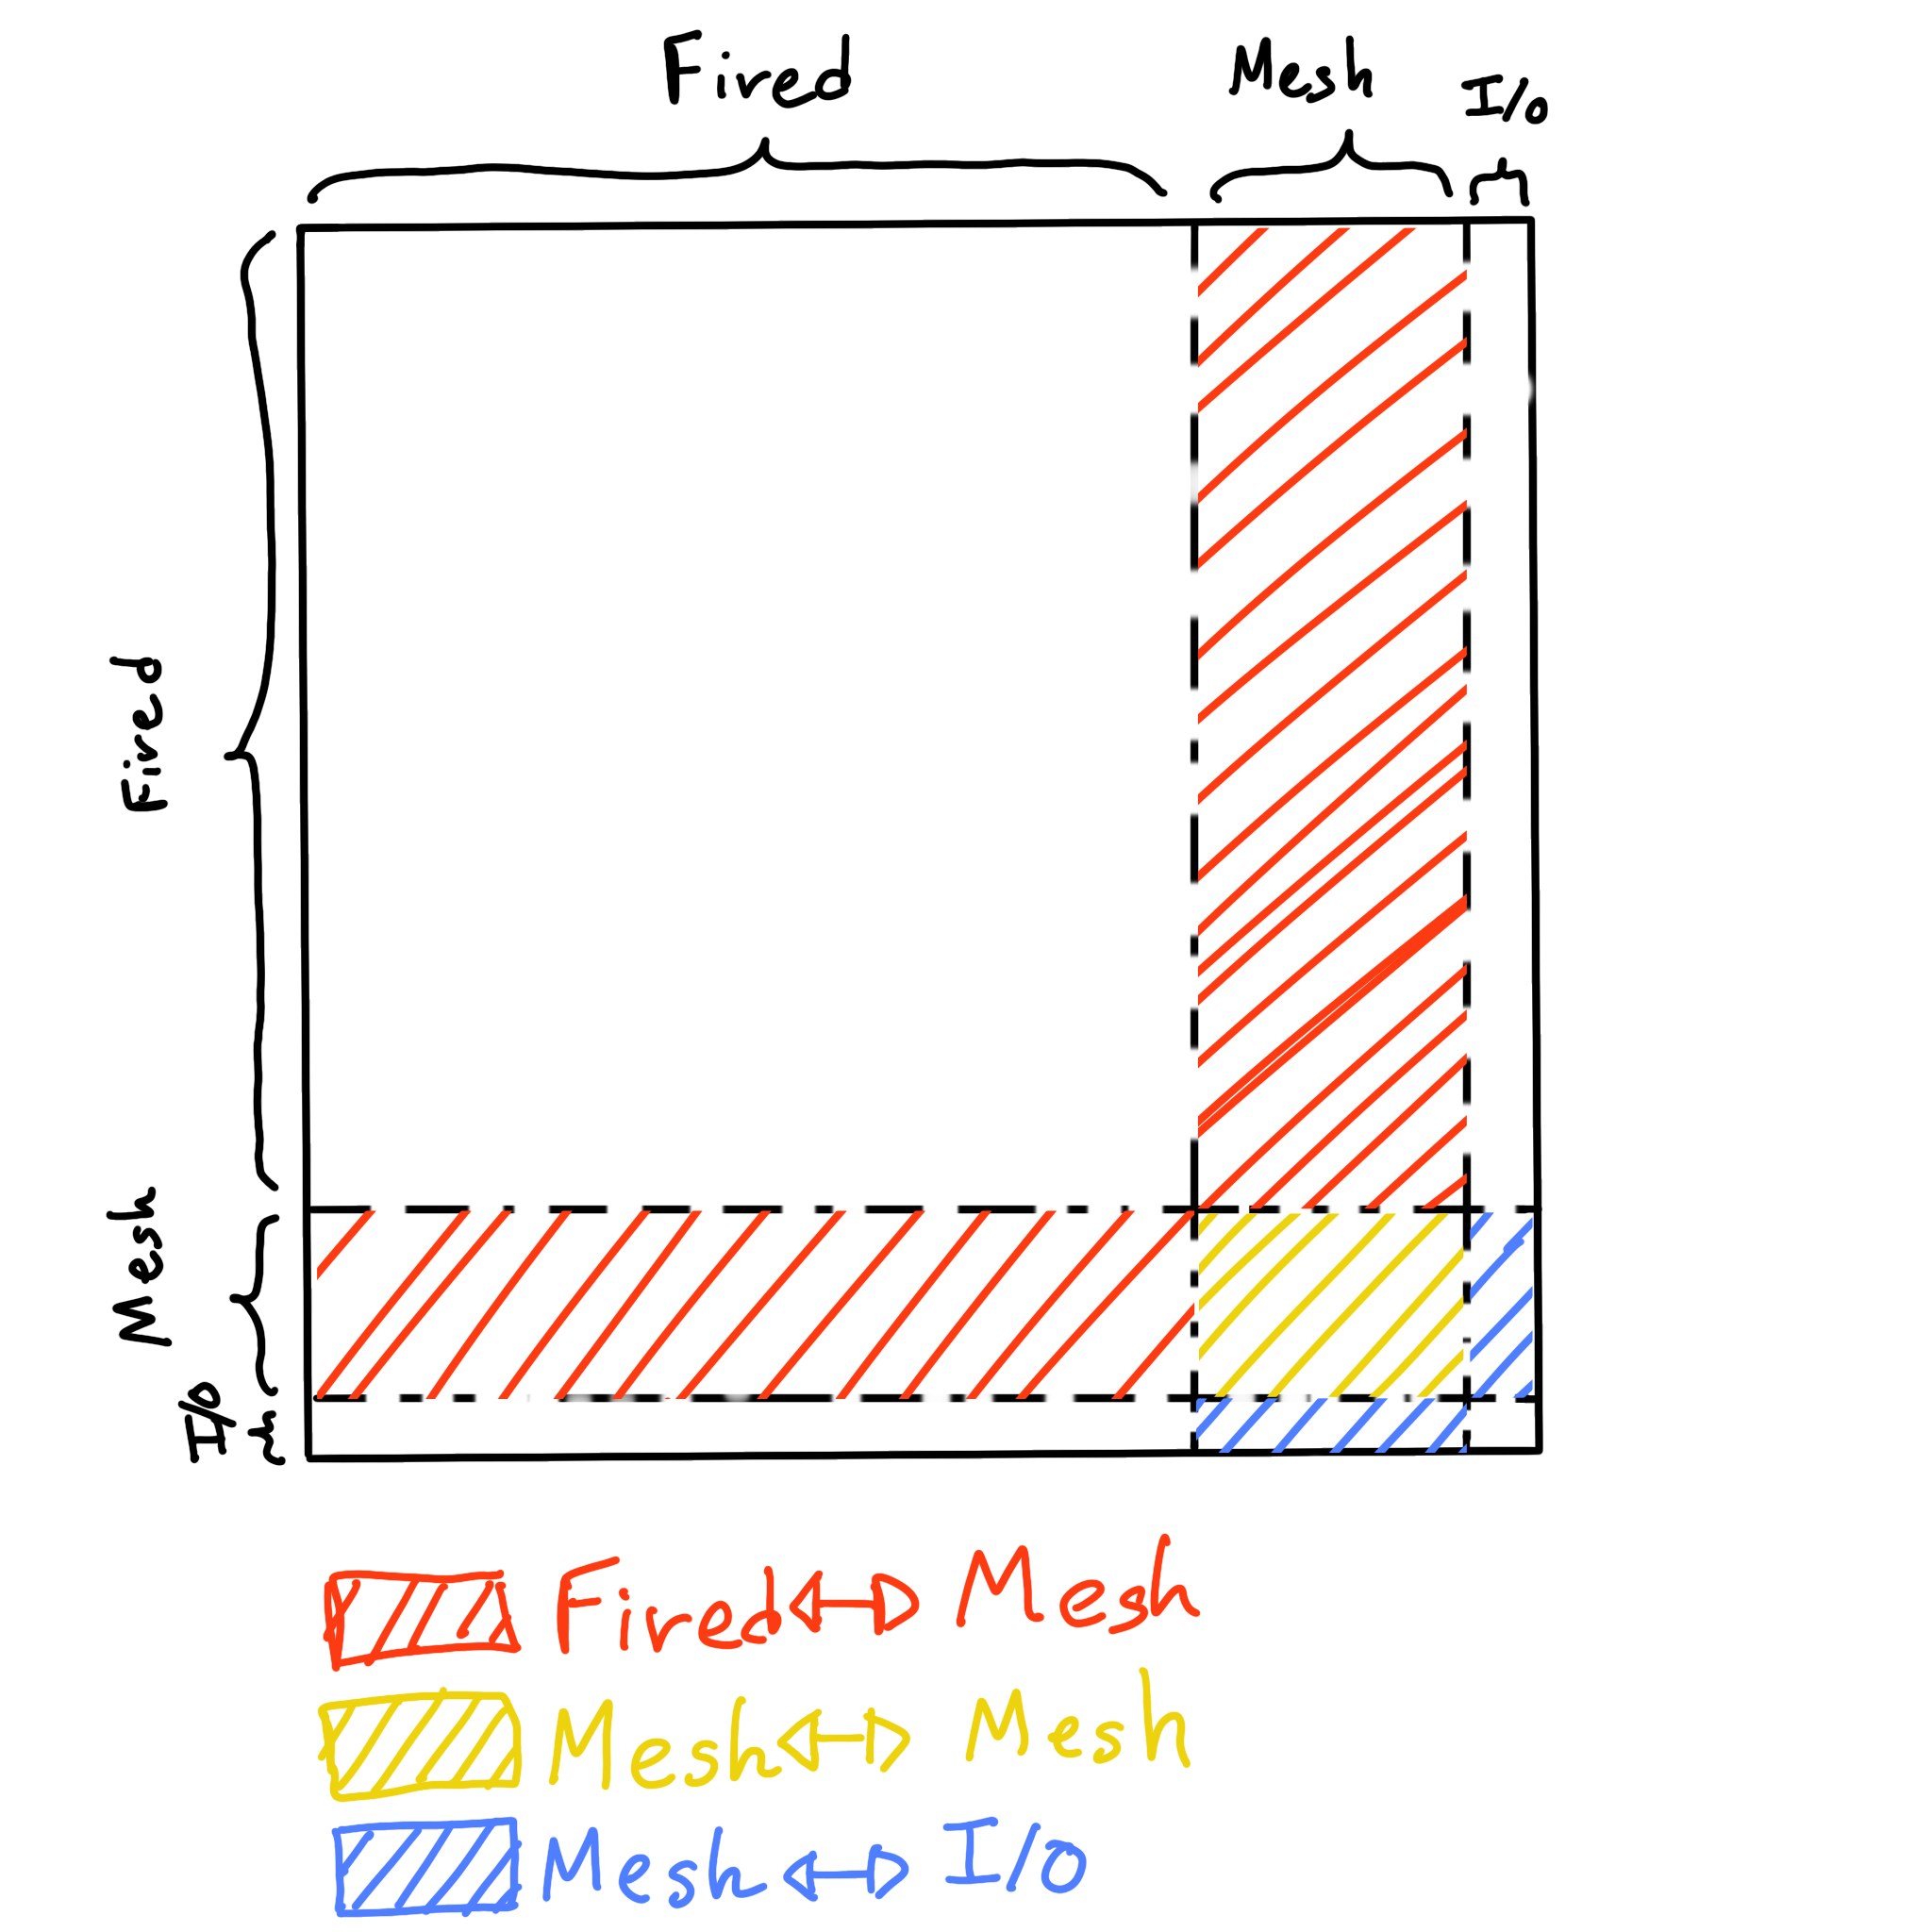
\includegraphics[width=\linewidth]{images/jgnn/adjacency_mat.png}
    \caption{Illustration of what a dense adjacency matrix would looks like and the part we a re really interested in. Because Fired $\rightarrow$ Mesh and Mesh $\rightarrow$ I/O relations are undirected, we only consider in practice the top right part of the matrix for those relations.}
    \label{fig:jgnn:adj}
  \end{subfigure}
  \caption{}
\end{figure}

\section{Message passing algorithm}
\begin{itemize}
  \item Need one message passing algorithm per connection (f->m, m->f, m->m, n->io, io->m)
  \item Allow to select part of the adjacency matrix (see notes)
  \item Explain message passing layer that was developed
  \item Reimplementation in C++ using torch framework
  \item C++ allow also for on the fly data transformation from raw file and minutieuse memory management
  \item Not updating the edge for the sake of technical simplicity: Commplicated to identify an edge feature from the above algorithm
\end{itemize}

\section{Data}
\begin{itemize}
  \item Present the data (dataset)
  \item Maybe show an example
\end{itemize}

\section{Model}
\begin{itemize}
  \item Present number of layers etc...
  \item Dicsucss hyperparamters optimisation
  \item Random search is not viable with the accessible hardware (too time consuming) -> 90h per trainng
  \item By hand optimization -> around 70 iterations and tests.
\end{itemize}

\section{Results}
Present the results

\section{Conclusion}
\begin{itemize}
  \item For now:
  \item Not competitive
  \item Aggregation on mesh nodes seems to loose informations
  \item Maybe too complex ?
  \item Next step would be to have the waveform dirrectly included
\end{itemize}

\end{document}
